%%%%%%%%%%%%%%%%%%%%%%%%%%%%%%%%%%%%%%%%%
% Beamer Presentation
% LaTeX Template
% Version 1.0 (10/11/12)
%
% This template has been downloaded from:
% http://www.LaTeXTemplates.com
%
% License:
% CC BY-NC-SA 3.0 (http://creativecommons.org/licenses/by-nc-sa/3.0/)
%
%%%%%%%%%%%%%%%%%%%%%%%%%%%%%%%%%%%%%%%%%

%----------------------------------------------------------------------------------------
%	PACKAGES AND THEMES
%----------------------------------------------------------------------------------------

\documentclass[aspectratio=169]{beamer} % Eliminate [aspectratio=169] to do narrow slides

\mode<presentation> {

% The Beamer class comes with a number of default slide themes
% which change the colors and layouts of slides. Below this is a list
% of all the themes, uncomment each in turn to see what they look like.

%\usetheme{default}
%\usetheme{AnnArbor}
%\usetheme{Antibes}
%\usetheme{Bergen}
%\usetheme{Berkeley}
%\usetheme{Berlin} 
%\usetheme{Boadilla} 
%\usetheme{CambridgeUS}
%\usetheme{Copenhagen}
%\usetheme{Darmstadt}
%\usetheme{Dresden}
%\usetheme{Frankfurt}
%\usetheme{Goettingen}
%\usetheme{Hannover}
%\usetheme{Ilmenau}
%\usetheme{JuanLesPins}
%\usetheme{Luebeck}
\usetheme{Madrid} 
%\usetheme{Malmoe}
%\usetheme{Marburg}
%\usetheme{Montpellier}
%\usetheme{PaloAlto}
%\usetheme{Pittsburgh}
%\usetheme{Rochester}
%\usetheme{Singapore}
%\usetheme{Szeged}
%\usetheme{Warsaw}

% As well as themes, the Beamer class has a number of color themes
% for any slide theme. Uncomment each of these in turn to see how it
% changes the colors of your current slide theme.

%\usecolortheme{albatross}
%\usecolortheme{beaver}
%\usecolortheme{beetle}
%\usecolortheme{crane}
%\usecolortheme{dolphin}
%\usecolortheme{dove}
%\usecolortheme{fly}
%\usecolortheme{lily}
%\usecolortheme{orchid}
%\usecolortheme{rose}
%\usecolortheme{seagull}
%\usecolortheme{seahorse}
\usecolortheme{whale}
%\usecolortheme{wolverine}

%\setbeamertemplate{footline} % To remove the footer line in all slides uncomment this line
%\setbeamertemplate{footline}[page number] % To replace the footer line in all slides with a simple slide count uncomment this line

\setbeamertemplate{navigation symbols}{} % To remove the navigation symbols from the bottom of all slides uncomment this line
}

\usepackage{graphicx} % Allows including images
\usepackage{booktabs} % Allows the use of \toprule, \midrule and \bottomrule in tables
\usepackage[export]{adjustbox}
\usepackage{blindtext}
\usepackage{hyperref}
\usepackage{graphicx}
\usepackage{amssymb}
\usepackage{amsmath}
\usepackage{bbm}
\usepackage{pgfplots}
\usetikzlibrary{intersections}
\pgfplotsset{compat=1.16}
\usepackage{tikz}
\usetikzlibrary{arrows.meta}
\usepackage[authoryear,round]{natbib}


%----------------------------------------------------------------------------------------
%	TITLE PAGE
%----------------------------------------------------------------------------------------

\title[Financial Frictions and Informality]{Financial Frictions and Informality} % The short title appears at the bottom of every slide, the full title is only on the title page

\author[David Morales]{\textbf{David Morales}}

\institute[TSE]{\textbf{Toulouse School of Economics}}


\date[November 2025] % (optional)
% {\textbf{Advisors}: Matteo Bobba \& Jean-Marie Lozachmeur\\
% \vspace{10mm}
{November 2025}

\begin{document}

\begin{frame}[noframenumbering]
\titlepage % Print the title page as the first slide
\end{frame}

%----------------------------------------------------------------------------------------
%	PRESENTATION SLIDES
%----------------------------------------------------------------------------------------



%------------------------------------------------

\begin{frame}
\frametitle{\textbf{Motivation}}
\textbf{Previous literature}:

\begin{itemize}
    \item Firms' credit access affect their decisions, including formality \textcolor{lightgray}{(\cite{amiti2018much,greenstone2020credit,gutierrez2023credit})}
    \vspace{5mm}
    \item Formality has multiple causes and consequences \textcolor{lightgray}{(\cite{ulyssea2018firms,meghir2015wages})}
    \vspace{5mm}
    \item Literature key takeaways:
    \begin{itemize}
        \item Credit access increases employment, productivity and firm entry, mainly among SMEs.
        \item Credit constraints are one of the main costs of informality. 
        \item Productivity distribution overlaps in the formal and informal sectors.
    \end{itemize}
\end{itemize}

\vspace{5mm}
\textbf{This paper}: Link of informality decisions and credit access.

\begin{itemize}
    \item What are the effects of financial constraints on firms decisions, particularly regarding informality?
\end{itemize}

\end{frame}

%------------------------------------------------

\begin{frame}
\frametitle{\textbf{Contribution}}

\textbf{Reduced-form}: \textcolor{gray}{\cite{gutierrez2023credit}, Berg (2018), \cite{greenstone2020credit}, Barbosa et al. (2019)}
\vspace{3mm}
\begin{itemize}
    \item \textbf{Contribution}: Analyse both the \textbf{extensive} and the intensive margins of informality.
\end{itemize}


\vspace{8mm}

\textbf{Job search models with financial frictions and/or informality}: \textcolor{gray}{\cite{flabbi2022working}, \cite{haanwinckel2021workforce}, \cite{meghir2015wages}, \cite{lise2013job}, \cite{krusell2010labour}}
\vspace{3mm}
\begin{itemize}
    \item \textbf{Contribution}: Center the analysis on firms rather than on workers' financial constraints. 
    \item \textbf{Contribution}: Explain capital distribution across formal status and its relation w/labor. 
\end{itemize}

\end{frame}

%------------------------------------------------

\begin{frame}
\frametitle{\textbf{Results}}

\begin{itemize}
    \item 1 s.d. credit supply shock in a market(CZ $\times$ sector) 3-months cumulative effect:
    \begin{itemize}
        \item +6.9\% amount of credits, +31.4 million pesos.
        \item +0.4\% formal workers, +1 formal worker.
        \item \textcolor{red}{?\%} informal workers \textcolor{red}{(In Progress...)}
        \item +0.2\% formal firms, +1 formal firm.
        \item -3.5\% informal firms, -4 informal firms.
        \item +0.2\% formal market wage bill, +6 thousand pesos.
        \item \textcolor{red}{?\%} informal market wage bill \textcolor{red}{(In Progress...)}
    \end{itemize}
\end{itemize}

\vspace{5mm}

\textbf{Heterogeneity}: This effects are concentrated on small firms.

\vspace{5mm}

\textbf{Possible explanation}: A credit shock induces infra-marginal informal firms to become formal.

\vspace{5mm}

\textbf{Model}: To identify the mechanism of the effect. 

\end{frame}

%------------------------------------------------

\begin{frame}
\frametitle{\textbf{Contribution}}
\label{contribution}


\textbf{Reduced-form}: \textcolor{gray}{\cite{gutierrez2023credit}, Berg (2018), \cite{greenstone2020credit}, Barbosa et al. (2019)}
\vspace{3mm}
\begin{itemize}
    \item \textbf{Contribution}: Analyse both the \textbf{extensive} and the intensive margins of informality.
\end{itemize}


\vspace{8mm}

\textbf{Job search models with financial frictions and/or informality}: \textcolor{gray}{\cite{flabbi2022working}, \cite{haanwinckel2021workforce}, \cite{meghir2015wages}, \cite{lise2013job}, \cite{krusell2010labour}}
\vspace{3mm}
\begin{itemize}
    \item \textbf{Contribution}: Center the analysis on firms rather than on workers' financial constraints. 
    \item \textbf{Contribution}: Explain capital distribution across formal status and its relation w/labor. 
\end{itemize}

% \hyperlink{back3}{\beamergotobutton{Back}}

% \textbf{Financial frictions and capital missallocation}: \textcolor{gray}{Moll (14)}

% \begin{itemize}
%     \item \textbf{Contribution}:
% \end{itemize}

% \textbf{Financial frictions and informality}: \textcolor{gray}{Flabbi and Tejada (2023), Haanwinckel and Soares (2021), Lise (13)}

% \begin{itemize}
%     \item \textbf{Contribution}:
% \end{itemize}

% \vspace{5mm}

% \textbf{Job search models with informality}: \textcolor{gray}{Meghir et al (2015)}

% \begin{itemize}
%     \item \textbf{Contribution}:
% \end{itemize}

% \vspace{5mm}


\end{frame}

%------------------------------------------------

\begin{frame}[noframenumbering]
\frametitle{}

\begin{center}
    \LARGE D A T A
\end{center}

\end{frame}

%------------------------------------------------

\begin{frame}{\textbf{Data}}

\begin{itemize}
    \item Matched bank-employer-employee data
    \begin{itemize}
        \item Novel measure of firms' formality, conditional on having a credit.
        \item 20 years of monthly data
        \item All formal workers and banking loans.
    \end{itemize}
    \vspace{5mm}
    \item Employment Survey
    \begin{itemize}
        \item Representative of the formal and informal sector. 
        \item Worker informality is 65\%.
    \end{itemize}
    \vspace{5mm}
    \item Economic Census
    \begin{itemize}
        \item Every 5 years (2009, 2014, 2019, \& 2024).
        \item Formal and informal firm level data.
    \end{itemize}
\end{itemize}



\end{frame}

%------------------------------------------------

\begin{frame}[noframenumbering]
\frametitle{}

\begin{center}
    \LARGE D E S C R I P T I V E \quad S T A T I S T I C S 
\end{center}

\end{frame}

%------------------------------------------------


\begin{frame}
\frametitle{\textbf{Loan's summary statistics}}

\begin{columns}[T]

    \begin{column}{0.4\textwidth} 
        \textbf{Data}: Business loans to individuals and legal entities
        \begin{itemize}
            \item \textbf{Years}: 2004-2024
            \item \textbf{Nb of firms}: 1,678,422
            \begin{itemize}
                \item \textbf{Context}: In 2019, 726,542 establishments got a credit (11.4\% of 6,373,169, EC).
            \end{itemize}
            \item \textbf{Nb of banks}: 127
            \item \textbf{Firm-Bank-year observations}: 3,001,320
            \pause
            \item \textbf{Problem}: Presence of limited mobility bias. Add de-bias technics. 
        \end{itemize}
    \end{column}

    \begin{column}{0.6\textwidth}
        \begin{center}
            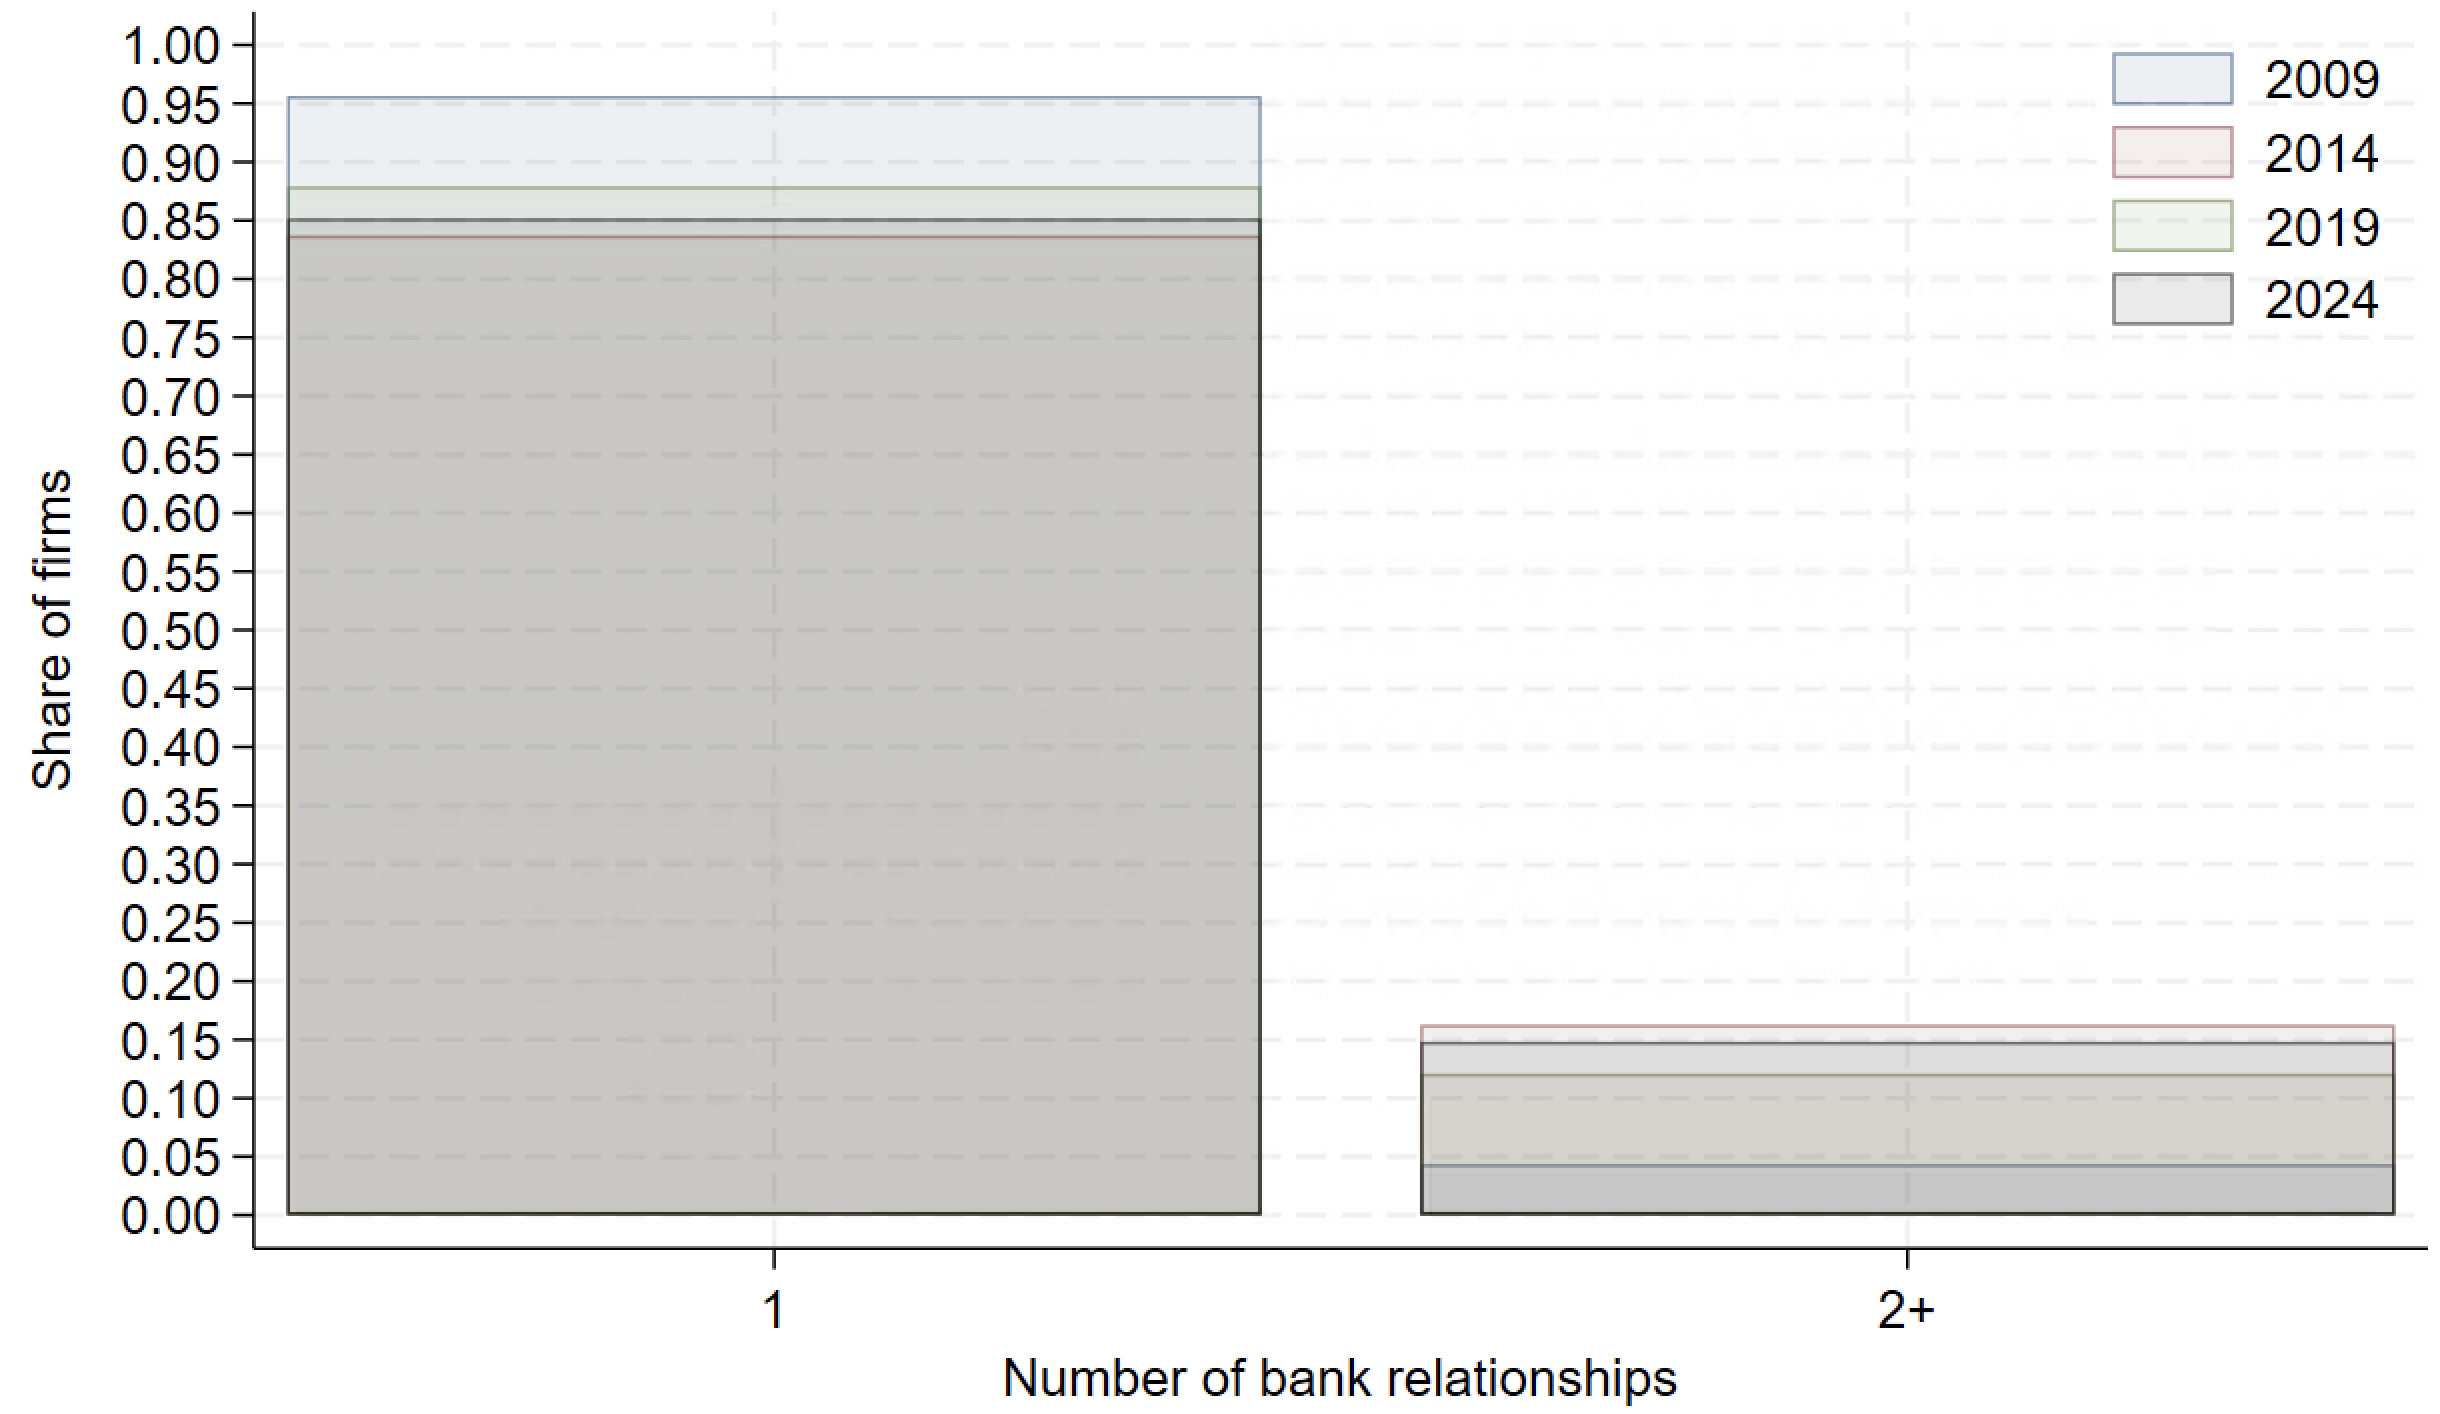
\includegraphics[scale=0.38]{hnbfirm.png}
        \end{center}
    \end{column}
    
\end{columns}

\end{frame}

%------------------------------------------------

% \begin{frame}
% \frametitle{\textbf{Variation on the total resources by year}} 

% \begin{center}
%     \includegraphics[scale=0.22]{totres0.png}
%     \includegraphics[scale=0.22]{totres1.png}
%     \includegraphics[scale=0.21]{totres2.png}
% \end{center}

% \end{frame}

%------------------------------------------------

\begin{frame}
\frametitle{\textbf{Bank concentration}} 

The level of bank concentration of new business loans varies widely over time

\vspace{5mm}

\begin{center}
    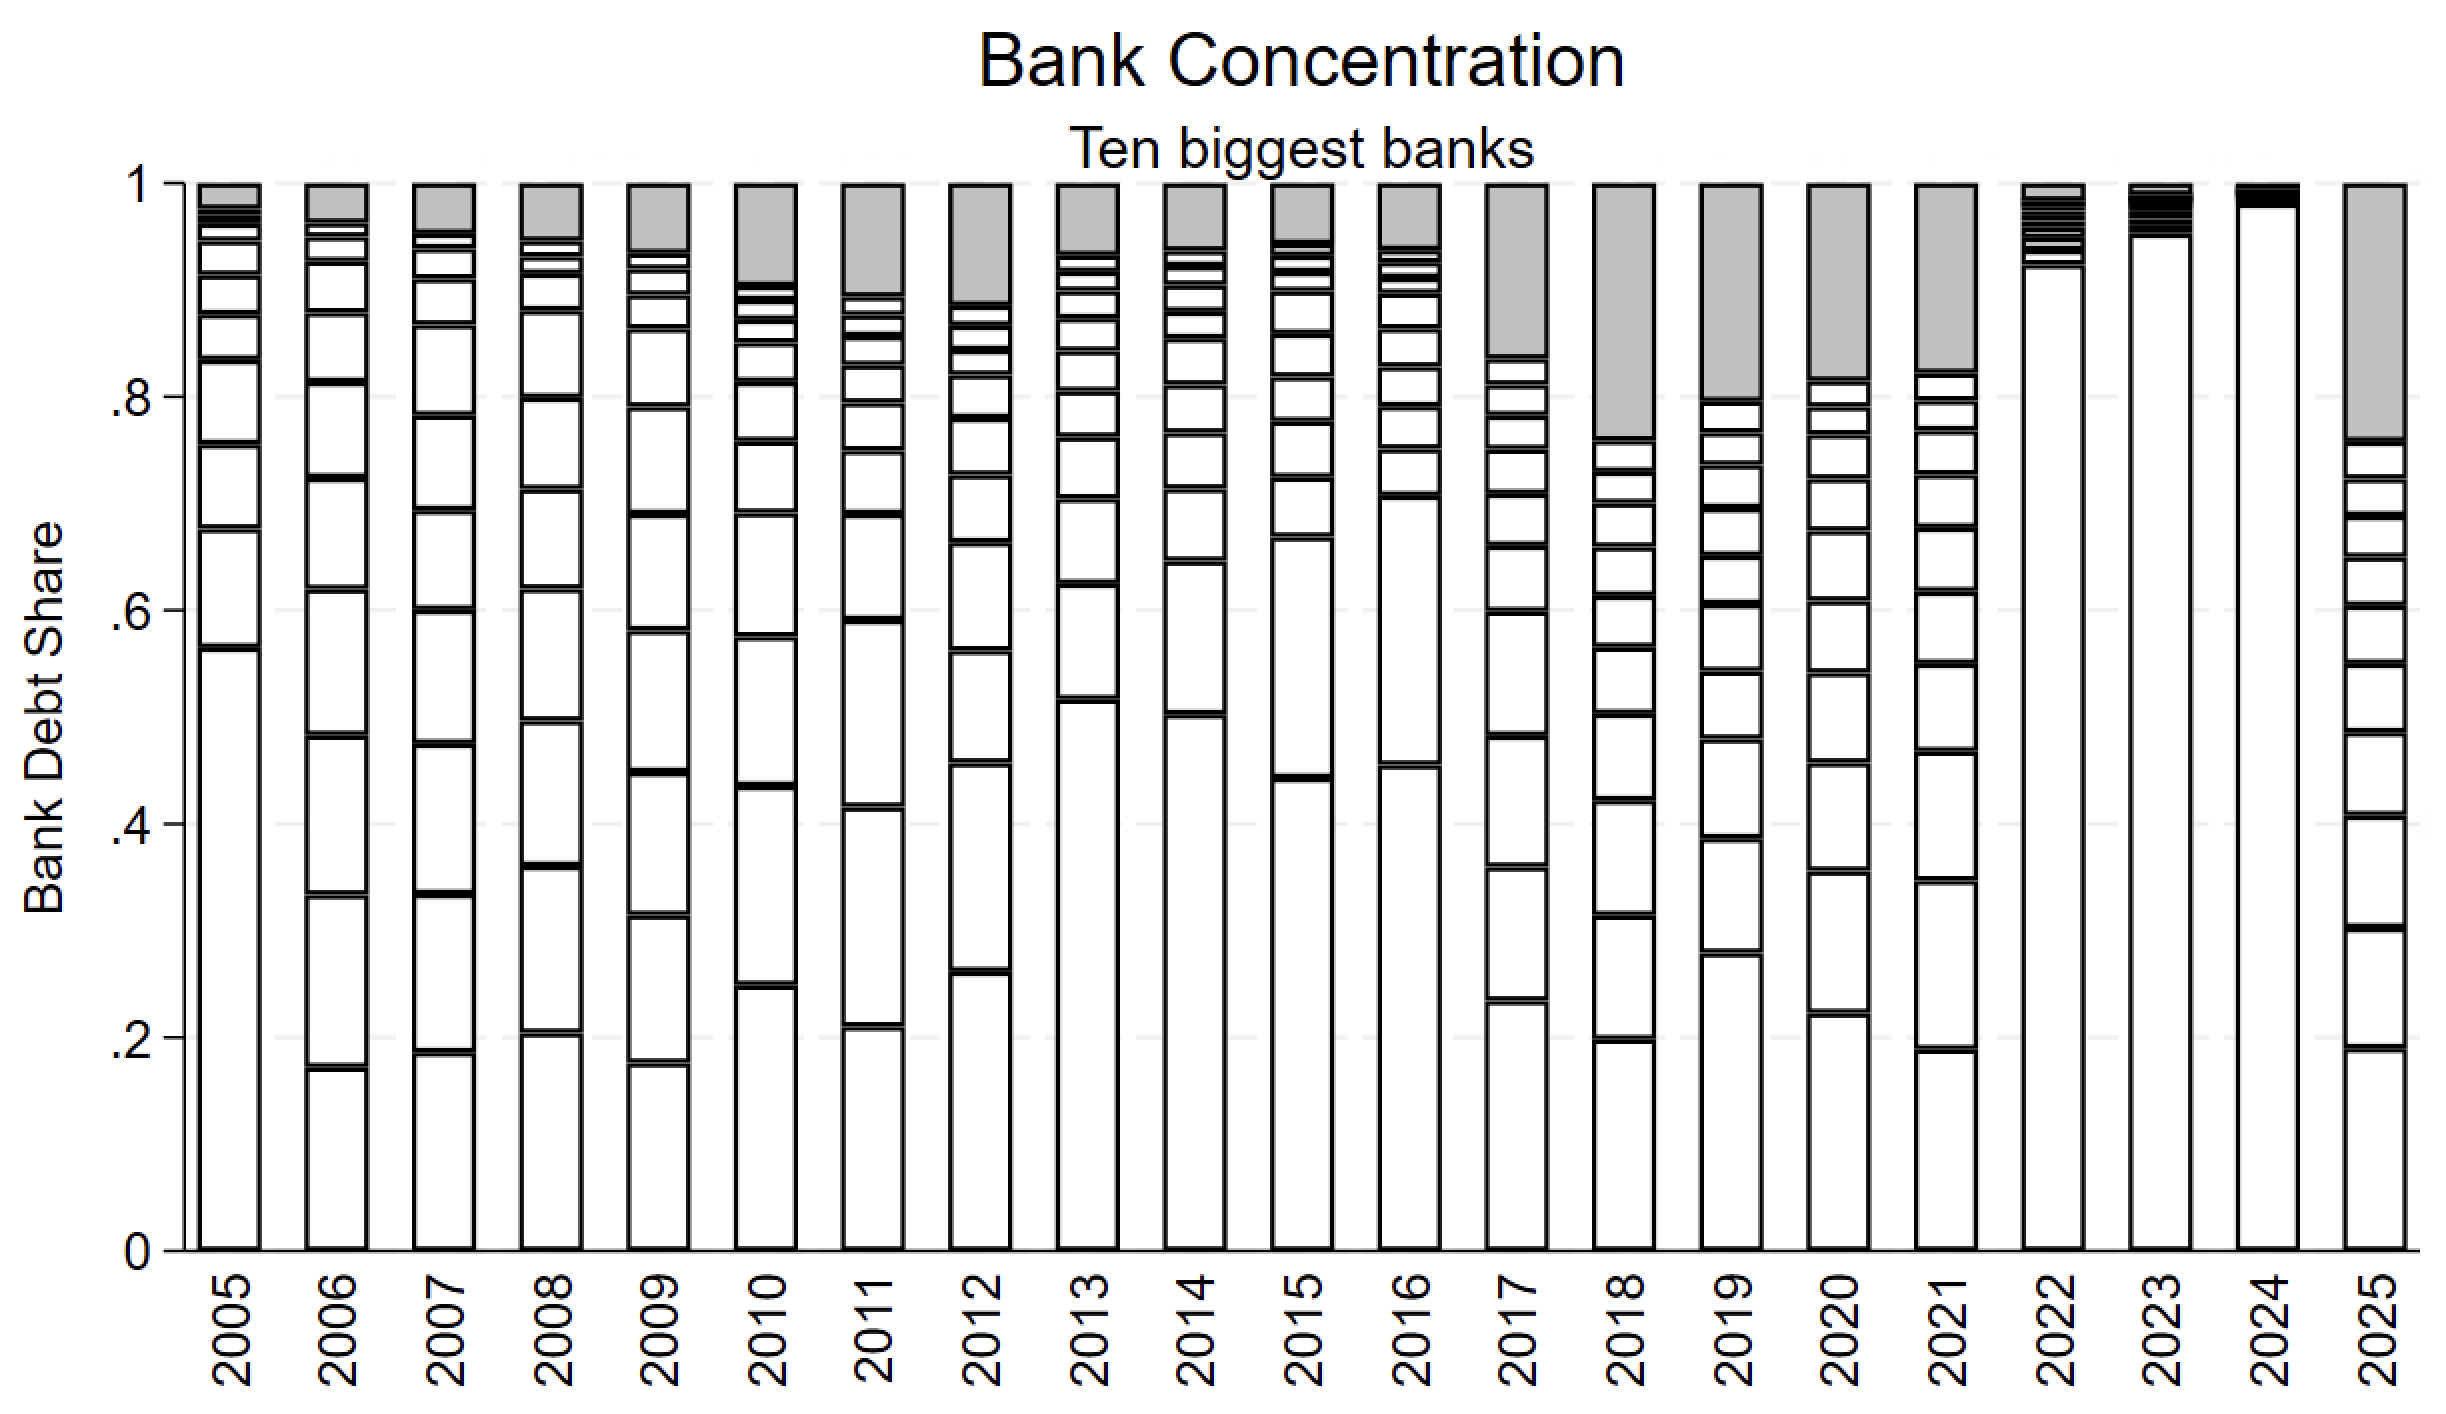
\includegraphics[scale=0.261]{10banks.png}
    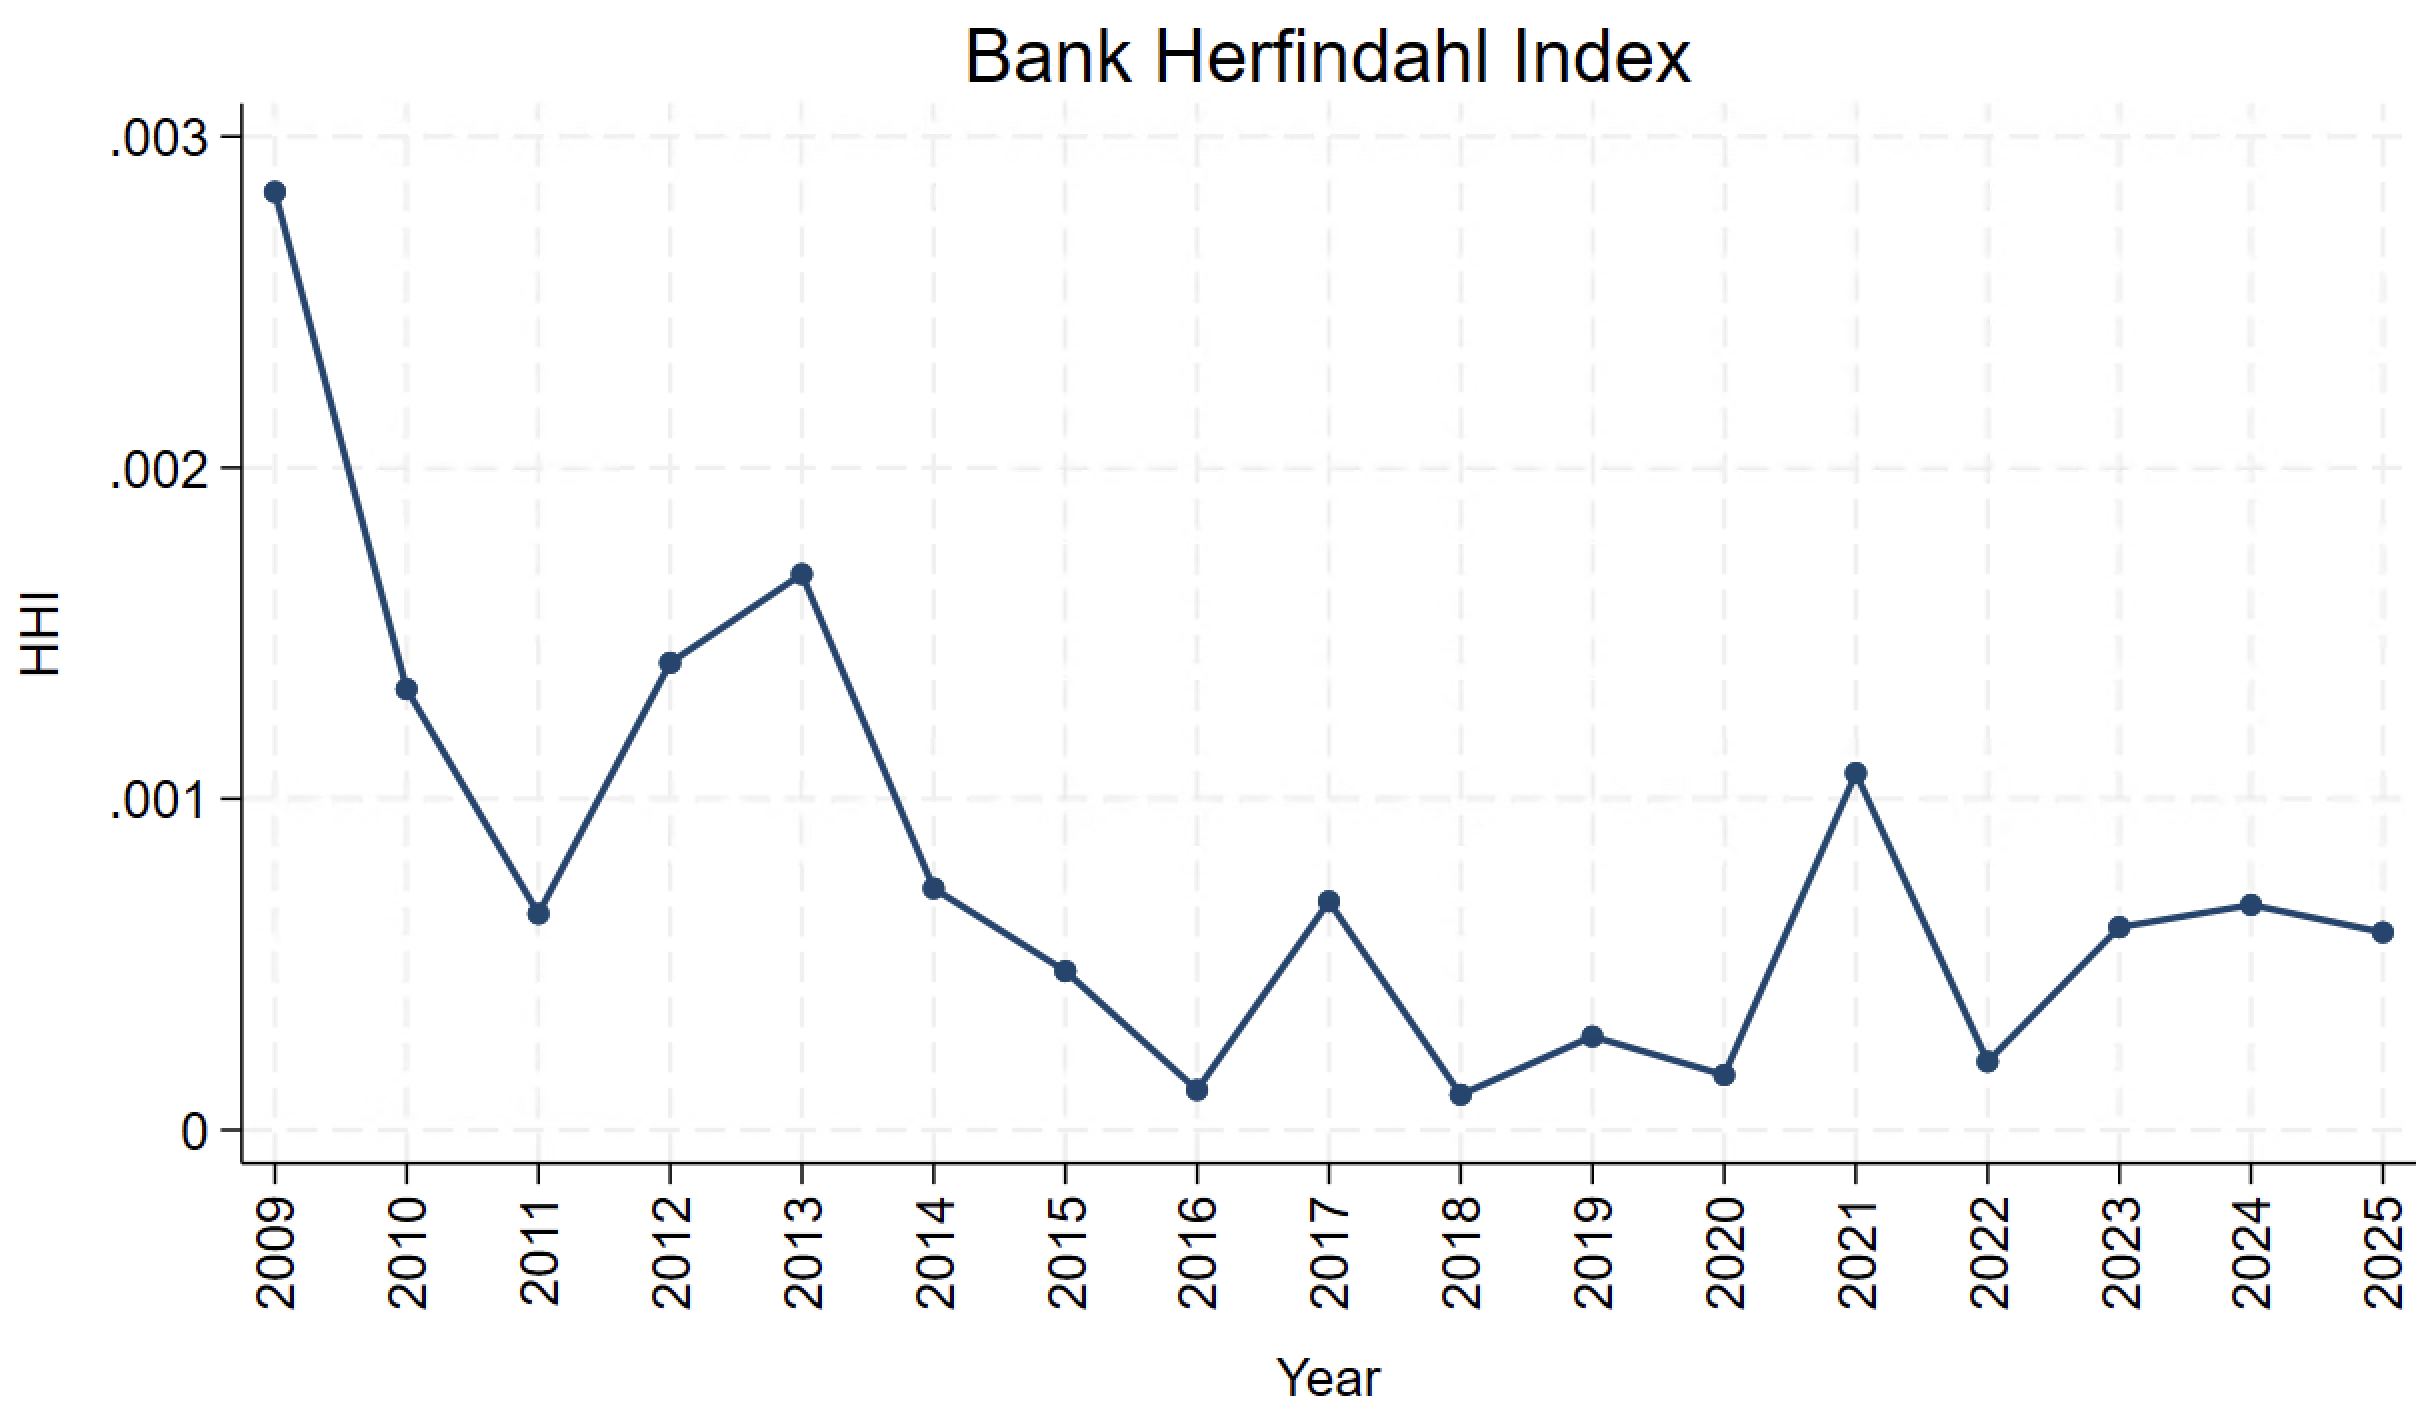
\includegraphics[scale=0.261]{hhibank.png}
\end{center}

\end{frame}

%------------------------------------------------

\begin{frame}
\frametitle{\textbf{Firm concentration}} 

The level of firm concentration of new business loans also changes over time

\vspace{5mm}

\begin{center}
    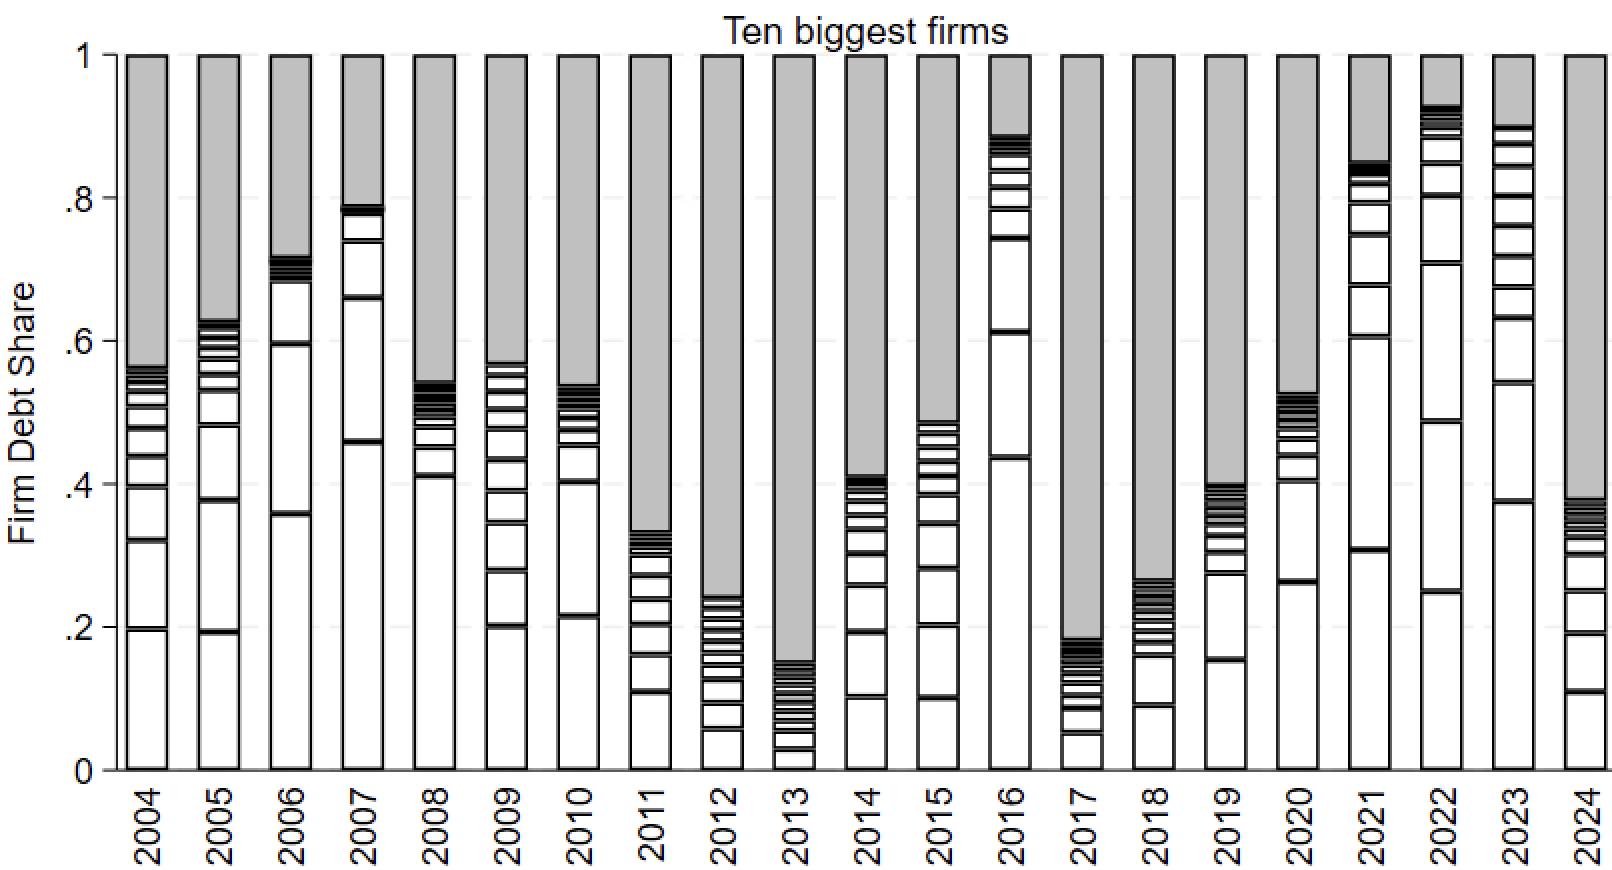
\includegraphics[scale=0.261]{10firms.png}
    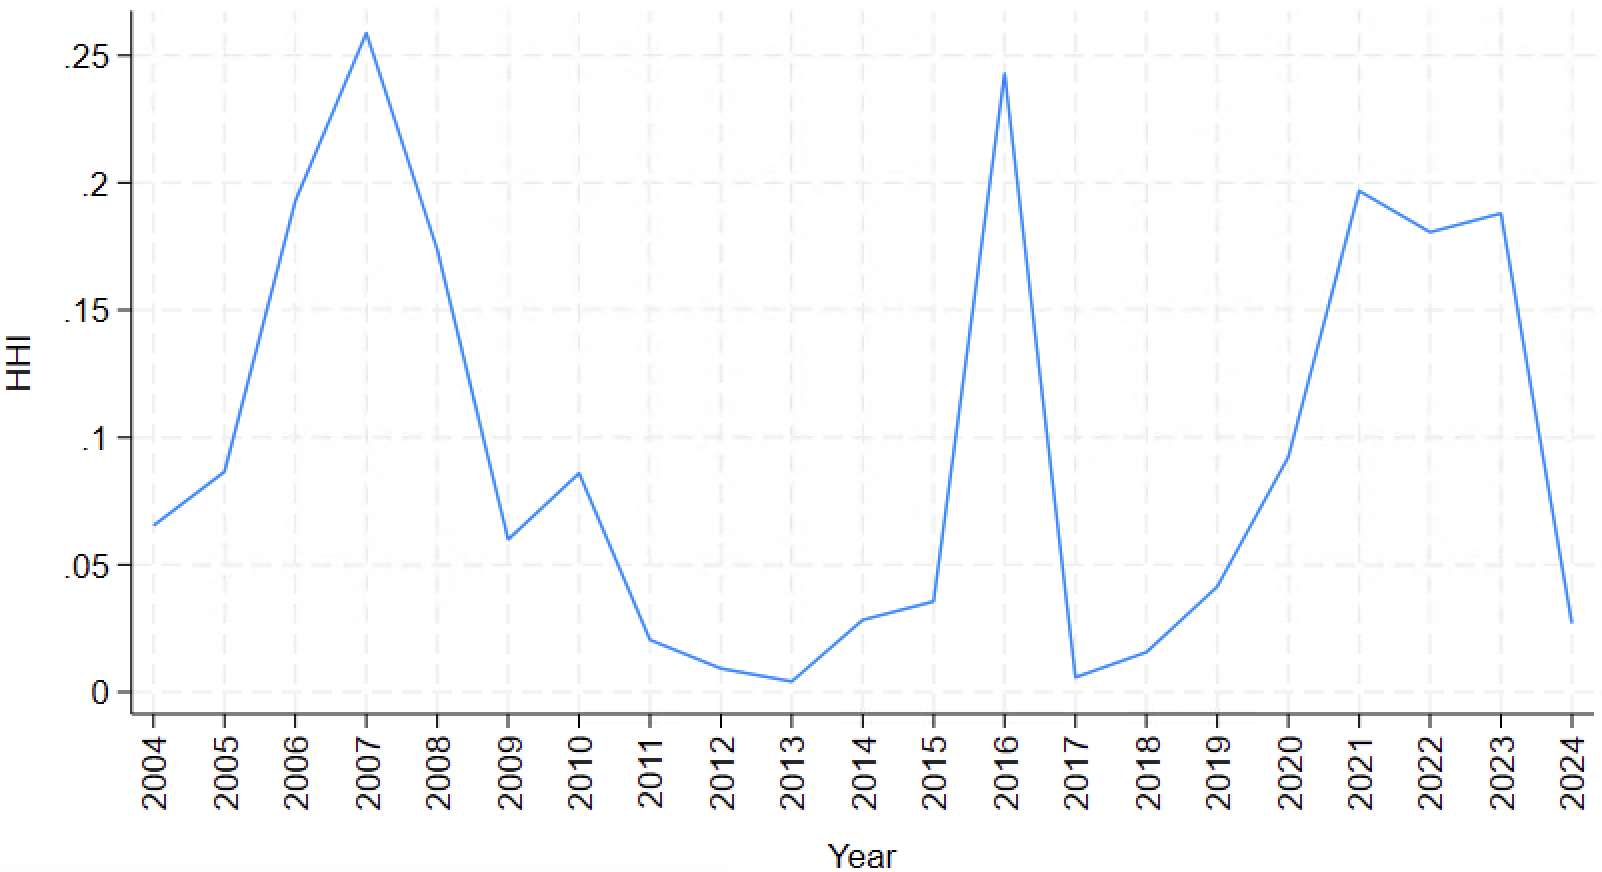
\includegraphics[scale=0.261]{hhifirm.png}
\end{center}

\end{frame}

%------------------------------------------------


\begin{frame}
\frametitle{\textbf{Firms formality transitions}} 

Current research focuses on Informal-Formal firm transition (\href{https://www.dropbox.com/scl/fi/njgwajjum07y6rk850uzf/DGMU_Final_Ecma.pdf?rlkey=ehlz6cvr0gdq9jyjoxsxwfzi6&e=1&dl=0}{Dix-Carneiro, Goldberg, Meghir, Ulyssea, Forthcoming ECMA}) or (\href{https://www.dropbox.com/scl/fi/8xy5ukqd9aswc7e5pxngh/0_Ecma_Main_Final.pdf?rlkey=qvzp0xnygfzz7fpwblgbbv2o1&e=1&dl=0}{Imbert, Ulyssea}). But Mexico Formal-Informal more relevant 
    \begin{center}
        \begin{table}[ht]
\centering
\caption{Firms transition between the formal and informal sectors}
\label{firms_transition}
\begin{tabular}{l*{1}{c}}
\hline\hline
Transition type          & Percent\\
\hline
Always formal            & 1.1\%  \\
Always informal          & 84.8\% \\
Formal-informal-formal   & 0.4\%  \\
From formal to informal  & 12.2\% \\
From informal to formal  & 1.1\%  \\
Informal-formal-informal & 0.3\%  \\
Total                    & 100\% \\
\hline\hline
\multicolumn{2}{l}{\footnotesize Source: Economic Census 2009, 2014, and 2019.}
\end{tabular}
\end{table}
    \end{center}
\end{frame}

%------------------------------------------------

\begin{frame}[noframenumbering]
\frametitle{}

\begin{center}
    \LARGE E M P I R I C A L \quad S T R A T E G Y
\end{center}

\end{frame}

%------------------------------------------------

\begin{frame}{\textbf{Empirical strategy}: Shift-Share à la \cite{greenstone2020credit}} \label{theory_shift}

\textbf{1) Decompose demand-supply effects}: Regress the change in bank-municipality log credit on bank, market and time fixed-effects:

\begin{equation*}
    \Delta \ln(C_{m,b,t}) = \alpha_{m,t} + \gamma_{b,t} + \epsilon_{m,b,t}
\end{equation*}

\vspace{3mm}

\pause

\textbf{2) Share}: Banks' share of total loans in a market in previous period:

\begin{equation*}
    s_{b,m,t-1} = \frac{L_{b,m,t-1}}{\sum_b L_{b,m,t-1}}
\end{equation*}

\vspace{3mm}

\pause

\textbf{3) Instrument}: Bank-level change in credit supply weighted by bank market share\footnote{Exposure-robust standard errors and Leave-one-out estimations following \cite{adao2019shiftshare}, \cite{krusell2010labour}, \cite{borusyak2022quasi}.}.

\begin{equation*}
    \hat{Z}_{m,t} = \sum_b \left( s_{b,m,t-1} \times \hat{\gamma}_{b,t} \right)
\end{equation*}

\end{frame}

%------------------------------------------------

\begin{frame}[noframenumbering]
\frametitle{}

\begin{center}
    \LARGE R E S U L T S
\end{center}

\end{frame}

%------------------------------------------------

\begin{frame}
\frametitle{\textbf{Evidence at firm level}: Bank and firm shocks} \label{back4}

There are \textbf{three periods of high variance} on the estimated shocks

\begin{center}
    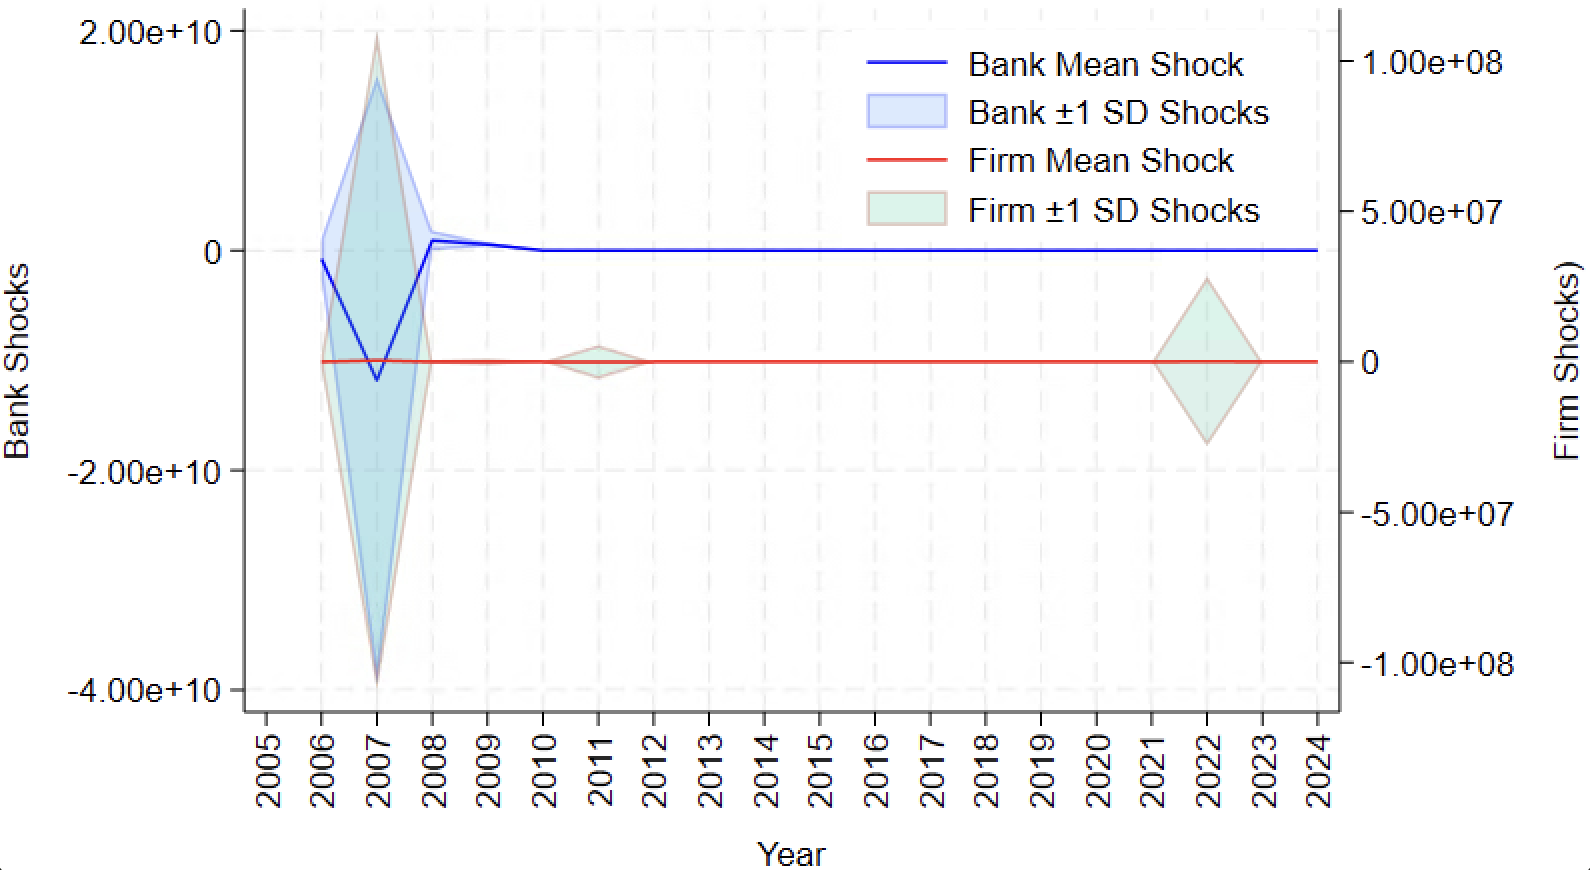
\includegraphics[scale=0.262]{CIshocks.png}
    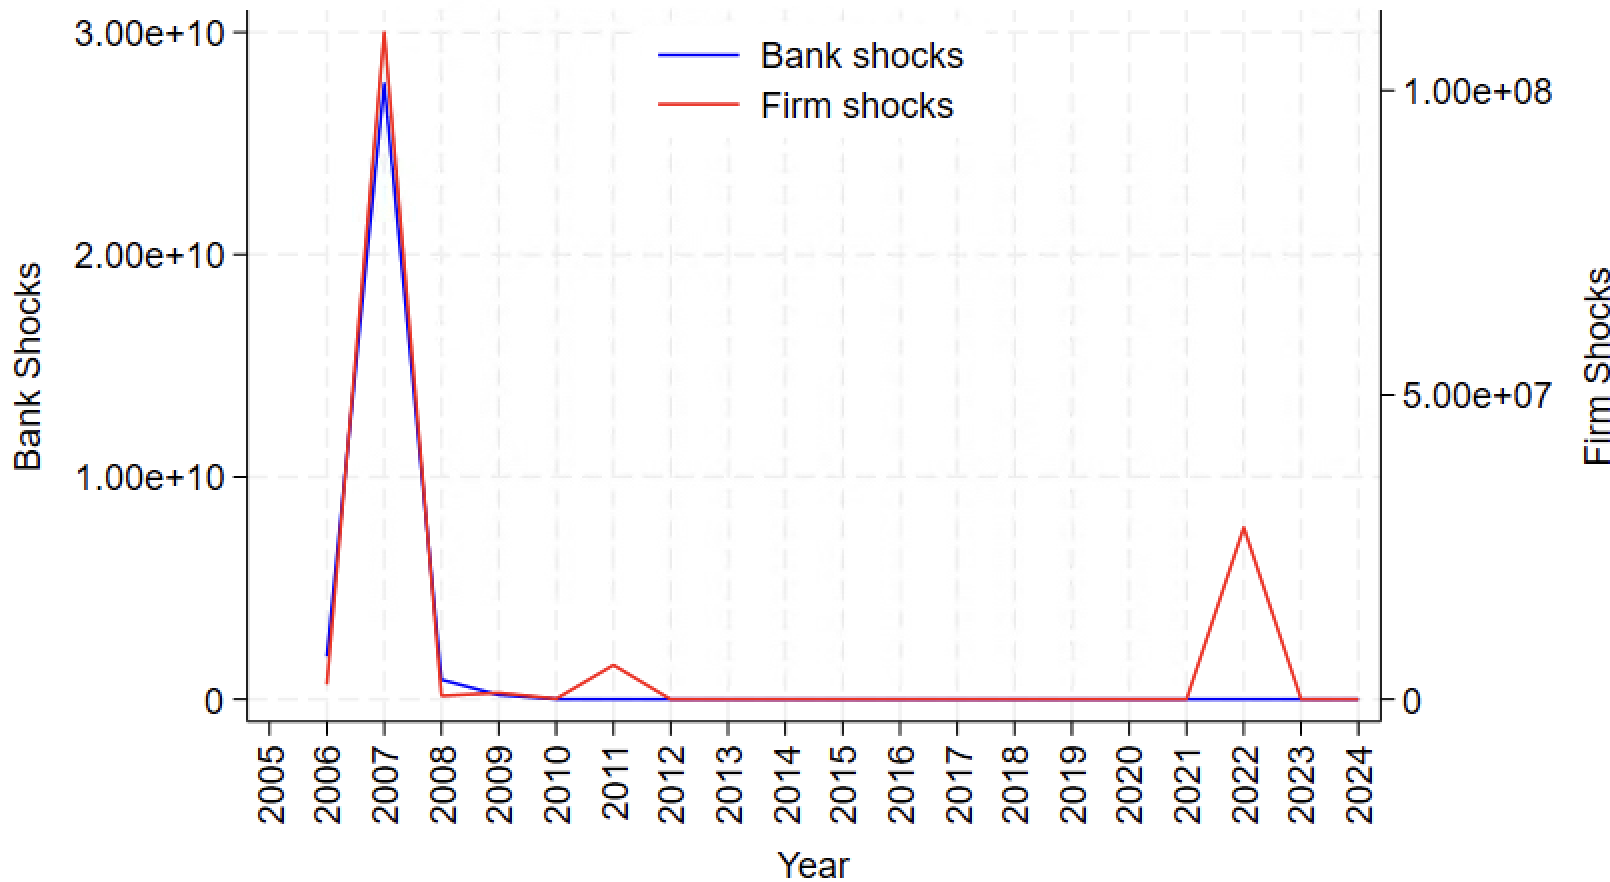
\includegraphics[scale=0.262]{SDshocks.png}
\end{center}

\hyperlink{sdsy}{\beamergotobutton{2012-2020}}

\end{frame}

%---------------------------------------------------

\begin{frame}{\textbf{Results}} 

\begin{table}[H]
\centering
\caption{Effect of standardized instrument on market-level log variables}
\label{shocks_activity}
\def\sym#1{\ifmmode^{#1}\else\(^{#1}\)\fi}
\begin{tabular}{l*{4}{c}}
\hline\hline
\hline
              & \multicolumn{3}{|c|}{Formal}  & Informal w/credit \\
              & \multicolumn{1}{|c}{Nb Workers} & Nb Firms & \multicolumn{1}{c|}{LLM Wage} & Nb Firm \\
\hline
Shock$_{t}$   & 0.001\sym{***} & 0.001\sym{***} & 0.001\sym{*}   & -0.014\sym{***}  \\
              & (0.0002)       & (0.0003)       & (0.0004)       & (0.002)          \\
[1em]
Shock$_{t-1}$ & 0.001\sym{***} & 0.001          & 0.001\sym{**}  & -0.013\sym{***}  \\
              & (0.0005)       & (0.0008)       & (0.0007)       & (0.002)          \\
Shock$_{t-2}$ & 0.002\sym{***} & 0.001\sym{***} & 0.001\sym{**}  & -0.008\sym{***}  \\
              & (0.0003)       & (0.0003)       & (0.0007)       & (0.001)          \\
\hline
Observations       & 100,110   & 100,110        & 100,110        & 153,280          \\
Adjusted-\(R^{2}\) & 0.9657    & 0.9697         & 0.9543         & 0.9745           \\
F-statistic        & 17.71     & 5.71           & 1.68           & 111.56           \\
Mean dep var       &14 (worker)& 429 (firm)     & 3.2 (M. pesos) & 102 (firm)       \\
\hline\hline
\multicolumn{5}{l}{\footnotesize Note: Standard errors are clustered at market level ($\approx$ 3,000 clusters).}\\
\end{tabular}
\end{table}

\end{frame}

%------------------------------------------------

\begin{frame}{\textbf{Results by size} 1/2} 

\begin{center}
    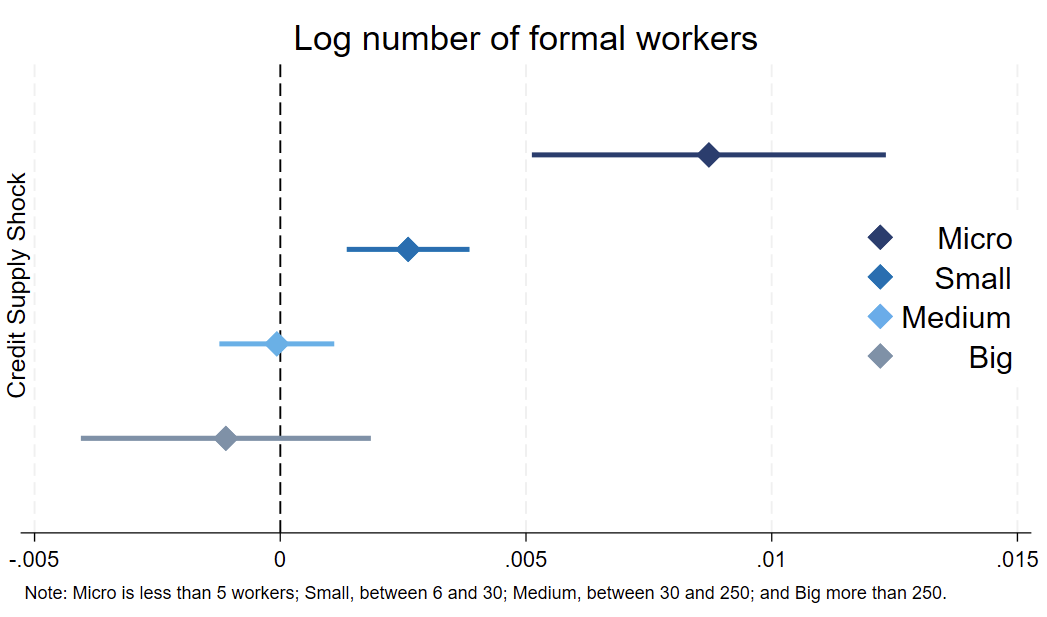
\includegraphics[scale=0.20]{size_f_workers.png}
    \pause
    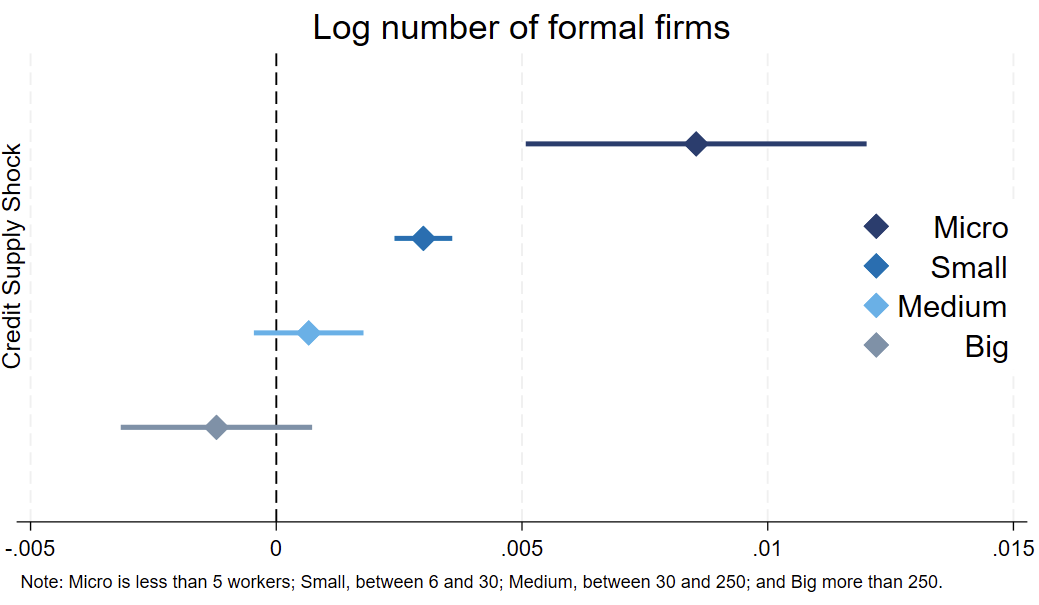
\includegraphics[scale=0.20]{size_f_firms.png}
\end{center}

\end{frame}

%------------------------------------------------

\begin{frame}{\textbf{Results by size} 2/2} 

\begin{center}
    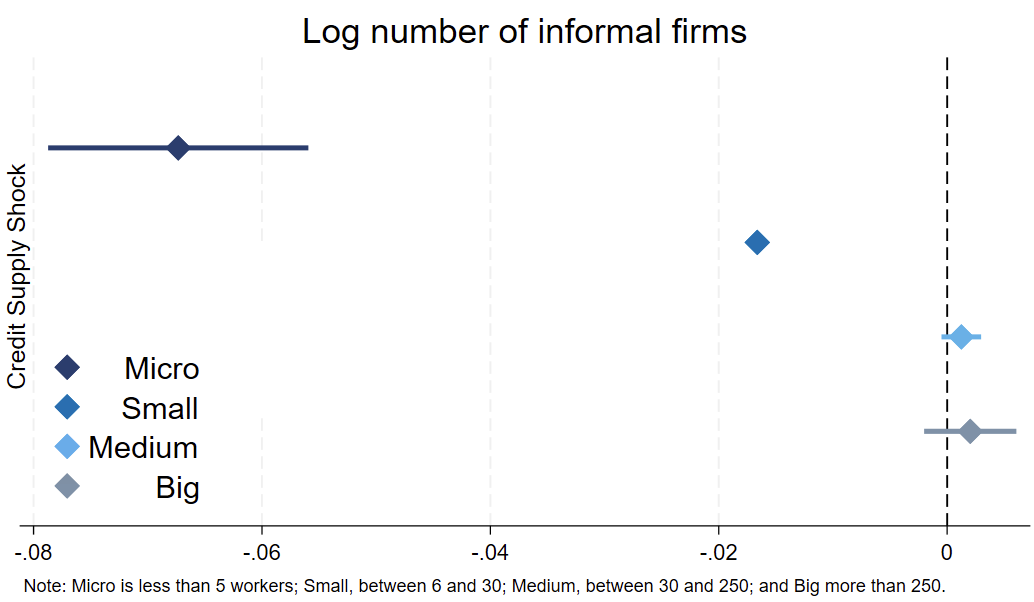
\includegraphics[scale=0.20]{size_i_firms.png}
    \pause
    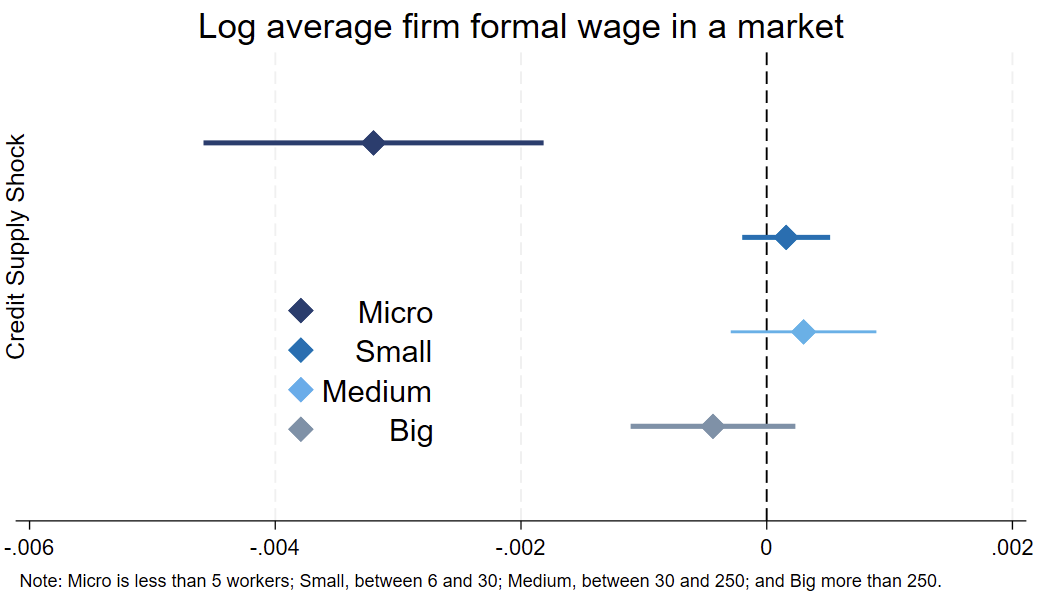
\includegraphics[scale=0.20]{size_f_wages.png}
\end{center}

\end{frame}

%------------------------------------------------

\begin{frame}[noframenumbering]
\frametitle{}
\begin{center}
    \LARGE M O D E L
\end{center}

\end{frame}

%------------------------------------------------

\begin{frame}
\frametitle{\textbf{Model}: Wage posting model w/capital and informality decisions}

\textbf{Setting}: 
\vspace{2mm}
\begin{itemize}
    \item \textbf{Firms}: Heterogeneous in productivity p, maximize firm's value.
    \pause
    \vspace{1mm}
    \item \textbf{Formality}: Affect profits and financial constraints. 
    \begin{itemize}
        \item If formal, profits' multiplicative term $B_f \mathbbm{1}_{\{f\}} \times \pi_{f}$, softer financial constraint $D < D^{max}_h$.
    \end{itemize}
    \pause
    \vspace{1mm}
    \item \textbf{Wage posting}: Same parameters for formal and informal sectors.
    \begin{itemize}
        \item Job destruction rate: $\gamma$, Job-offer arrival rate: $\lambda_1$, Wage offer distributions: $F(w)$.
    \end{itemize}
\end{itemize}
\pause
\vspace{3mm}

\textbf{Timing}: 
\vspace{2mm}
\begin{enumerate}
    \item \textbf{Period 1}: Decide the extensive margin of formality ($h = \{f=Formal,i=Informal\}$).
    \pause
    \vspace{1mm}
    \item \textbf{Period 2}: Decide next period capital ($k^h_2$), dividends to pay ($d^h_1$), and debt level ($D^h_1$).
    \pause
    \vspace{1mm}
    \item \textbf{Period 3}: Debt repayment +  Continuous time wage posting environment.
\end{enumerate}

\vspace{3mm}

% \textbf{Notice}: 

% \begin{itemize}
%     \item It will be solved backwards.
% \end{itemize}

\end{frame}

%------------------------------------------------

\begin{frame}
\frametitle{\textbf{Model}: Period 3}

\only<1>{\textbf{Problem}: Taking everything else as given, a firm decides a \textbf{wage} ($w$) to post:
\begin{equation*}
    \max \limits_{\{ w^h \}} \quad \left[ p*L(w^h) \right] ^{(1-\alpha)} \left[ k^{h} \right]^{\alpha} - w^hL(w^h) - (1+r)D^{*h}
\end{equation*}}


\only<2>{\textbf{Optimal wage posted}: Optimized $k_2^*$ in the previous period is taken as given.

\vspace{-6mm}

% \begin{equation*}
%     w^{*h}(p,\textcolor{blue}{k_2^{*h}}) = \underbrace{\textcolor{blue}{(1-\alpha) \biggr[k_2^{*h} \overbrace{\frac{[\gamma + \lambda \Bar{F}(w)]^{2}}{(\gamma(\gamma + \lambda))}}^{= 1/L^h(w)} \biggr]^{\alpha}} p^{\textcolor{blue}{(1-\alpha)}}}_{\text{MPL}} + \underbrace{\frac{[\gamma + \lambda \Bar{F}(w)]}{2 \lambda f(w)}}_{\text{Equilibrium effect}}
% \end{equation*}

\begin{multline*}
    w^{*h}(x, k_2^{*h}) = \underbrace{\textcolor{blue}{\left(\frac{k^{*h}}{L^h}\right)^\alpha}}_{\text{K per worker}} \left[ \underbrace{p^{\textcolor{blue}{(1 - \alpha)}}}_{\text{L-productivity}} - \\
    \underbrace{\textcolor{blue}{(1 - \alpha)} \left(\gamma + \lambda_1 \overline{F}_p(p)\right)^{2\textcolor{blue}{(1-\alpha)}}\int^p_{\underline{p}} \frac{dx}{\textcolor{blue}{x^{\alpha}} [\gamma + \lambda_1 F_p(x)]^{2\textcolor{blue}{(1-\alpha)}}} }_{\text{Equilibrium effect}} \right] 
\end{multline*}

% \begin{multline*}
%     w^{*h}(x, k_2^{*h}) = \underbrace{p^{\textcolor{blue}{(1-\alpha)}} \textcolor{blue}{(k^{*h} \overbrace{\frac{[\gamma + \lambda_1 \overline{F}_p(w)]^2}{\gamma (\gamma + \lambda_1)}}^{1/L(w)})^{(\alpha)}}}_{\text{Marginal Product of Labor}} - \\
%     \underbrace{\textcolor{blue}{(1-\alpha) (\frac{k_2^{*h}}{\gamma(\gamma + \lambda_1)})^{\alpha}} [\gamma + \lambda_1 \overline{F}_p(p) ]^2 \int^p_{\underline{p}} \frac{dx}{x^{\alpha} [\gamma + \lambda_1 F_p(x)]^{2(1-\alpha)}}}_{\text{Equilibrium effect}}
% \end{multline*}

\vspace{2mm}

\begin{itemize}
    \item The difference with the standard wage posting is in \textcolor{blue}{blue}. \textbf{Why does it matter?} 
    \begin{itemize}
        % \item All p-k-type firms (same capital and productivity) will post a unique wage $w(p,k_2^*)$.
        \item Firm becomes \textcolor{blue}{p-k-type} that depends on productivity and capital. 
        % \pause
        % \item Given capital (productivity), wage differences due to productivity (capital) differences.
    \end{itemize}
    % \item Wage is increasing in both productivity (p) and chosen capital ($k_2^{*h}$).
    % \begin{itemize}
    %     \item \textbf{Implication}: $ F(w(p,k_2^{*h})) = H(p,k_2^{*h}) $.
    % \end{itemize}
\end{itemize}}


\end{frame}

%------------------------------------------------

\begin{frame}
\frametitle{\textbf{Model}: Period 2}

\only<1>{\textbf{Problem}: Given formality, productivity, and wage ($w^*$), firm decides \textbf{capital} ($k_2$) \& \textbf{debt} ($D$):
\begin{align*}
    \max \limits_{\{ k_2, D \}} \Pi^h (w^{*h},p,k_2,D) & = B_f \mathbbm{1}_f \cdot \pi^h_1(w^{*h},p,k_1) - I^h + \beta [\pi^h_2(w^{*h},p,k_2) - (1 + r)D] \\
    s.t.: k_2^h & = I^h + (1-\delta) k_1 + D \\
    D & < D^{max}_h % = \theta_f k 
\end{align*}}

\only<2>{\textbf{Optimal capital}:
\begin{equation*}
    \underbrace{\alpha \biggr(\frac{k_2^{*h}}{pl}\biggr)^{(\alpha - 1)} + \overbrace{w'_{k_2^{*h}}(p,k_2^{*h})L^h}^{\text{Wage posting behaviour}}}_{\text{Marginal gain}} = \underbrace{\frac{1}{\beta}}_{\text{Marginal cost}}
    % \alpha \biggr(\frac{pl}{k_2^*}\biggr)^{(1 - \alpha)} + w'_{k_2^*}(p,k_2^*)l - (1-\delta) = \frac{1}{\beta}
\end{equation*}
% \begin{equation*}
%     k_2^* =  \biggr[\frac{1-\beta(1-\delta))}{\alpha \beta p} \frac{[\delta + \lambda\Bar{F}(w^*)]^2}{\delta + \lambda} + (\frac{p}{k_2^*})^{1-\alpha} + \frac{A}{\alpha}) \biggr]^{1/(\alpha - 1)}
% \end{equation*}

\begin{itemize}
    % \item Marginal gain equal marginal cost, internalizing the change in the wage posting behavior.
    \item Under certain conditions, $k_2^{*h}$ is increasing in productivity $p$.
\end{itemize}}

\only<3>{\textbf{Optimal debt level}:
\begin{equation*}
    D^{*h} \begin{cases}
        = 0 & \text{if profits $\geq$ cost of k: } \textcolor{lightgray}{k_2^{*h} - (1 - \delta)k_1 \leq I^{max} = \pi^h_1(w^{*h},p,k_1)} \\
        = k_2^{*h} - (1 - \delta)k_1 & \text{if profits $\leq$ cost of k $\leq$ max debt: } \textcolor{lightgray}{k_2^{*h} - (1 - \delta)k_1 \leq I^{max}_h + D^{max}_h} \\
        = D^{max}_h & \text{if cost of k $\geq$ max debt: } \textcolor{lightgray}{k_2^{*h} - (1 - \delta)k_1 > I^{max}_h + D^{max}_h}
    \end{cases}
\end{equation*}}

\end{frame}

%------------------------------------------------

\begin{frame}
\frametitle{\textbf{Model}: Period 1}


\textbf{Optimal (extensive) formality decision}: Given profits are strictly increasing functions of p, there exists a unique threshold $\tilde{p}$ where both profits are equal.

\begin{equation*}
    \text{Formal firm if } \Pi^{f} (w^{*f},p,k^{*f}_2,D^{*f}) = \Pi^{i} (w^{*i},p,k^{*i}_2,D^{*i}) \Leftrightarrow p = \tilde{p}
\end{equation*}

\vspace{3mm}

\begin{columns}[T] 
    \begin{column}{0.5\textwidth} 
        \centering
        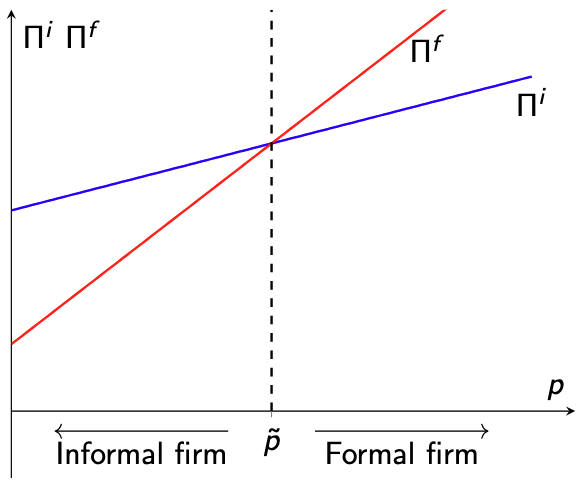
\includegraphics[scale=0.25]{gra2.png}
    \end{column}

    \pause

    \begin{column}{0.5\textwidth} 
    \textbf{Implications}
        \begin{itemize}
            \item More productive firms
            \begin{itemize}
                \item Pay higher wages.
                \item Have a bigger labor force.
                \item Hold more capital.
                \item Allocate in the formal sector. 
            \end{itemize}
        \end{itemize}

        \pause
        
        \vspace{5mm}
        \textbf{But what about the financial constraint?}
    \end{column}
\end{columns}


\end{frame}

%------------------------------------------------

\begin{frame}[noframenumbering]
\frametitle{}

\begin{center}
    \LARGE M A I N \quad I M P L I C A T I O N
\end{center}

\end{frame}

%------------------------------------------------


\begin{frame}
\frametitle{\textbf{Model main implication}}

\textbf{Implication}: A p-k-type informal firm becomes a p-k'-type formal firm wo/the constraint ($k' > k$).

\vspace{3mm}

\begin{center}
    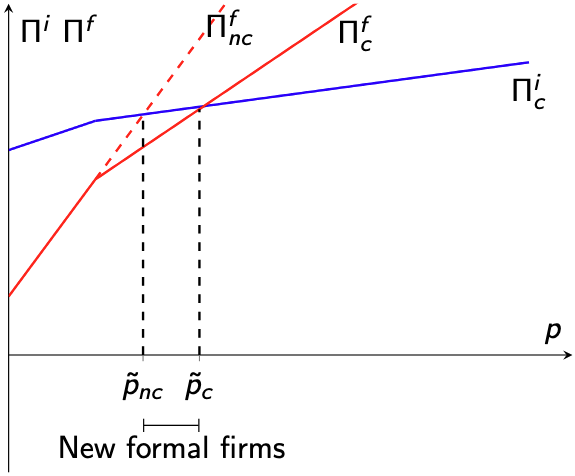
\includegraphics[scale=0.25]{gra3.png}
\end{center}

\pause

\textbf{Testable}: It can be tested in the data with changes in financial constraints of firms.


\end{frame}

%-----------------------------------------------

\begin{frame}[noframenumbering]
\frametitle{}
\begin{center}
    \LARGE S I M U L A T E D \quad M O D E L
\end{center}

\end{frame}

%------------------------------------------------

\begin{frame}
\frametitle{Model simulation}

\textbf{Preliminary values for parameters}:

\begin{columns}[T] 
    \begin{column}{0.5\textwidth} 
        \begin{itemize}
            \item \textbf{Interest rate}: $r = 0.05 \Rightarrow \beta = 0.95$.
            \item \textbf{Depreciation rate}: $\delta = 0.1 $.
            \item \textbf{Destruction rate}: $\delta_e = 0.2 $.
            \item \textbf{Arrival rate if unemployed}: $\lambda_0 = 0.7 $.
            \item \textbf{Arrival rate if employed}: $\lambda_1 = 0.4 $.
            \item \textbf{Informality cost} (mult.): $B_i = 0.9 $.
        \end{itemize}
    \end{column}

    \begin{column}{0.5\textwidth} 
        \begin{itemize}
            \item \textbf{Weight on capital}: $\alpha = 0.5$.            
            \item \textbf{Share  of informal firms}: 58\%.
            \item \textbf{Max debt if formal}: $D^i_{max} = 3,000$.
            \item \textbf{Max debt if informal}: $D^f_{max} = 800$.
            \item \textbf{Distribution of wages}: From real data.
            \item \textbf{Endowment if formal}: $\pi^f_0 = 3,100$.
            \item \textbf{Endowment if informal}: $\pi^i_0 = 3,700$.
        \end{itemize}
    \end{column}
\end{columns}

\end{frame}

%------------------------------------------------

\begin{frame}
\frametitle{\textbf{Simulated model} 1/2}

\vspace{-10mm}

\begin{columns}[T] 
    \begin{column}{0.5\textwidth} 
        \begin{center}
            \textbf{Debt}
        \end{center}
        \vspace{-5mm}
        \begin{center}
            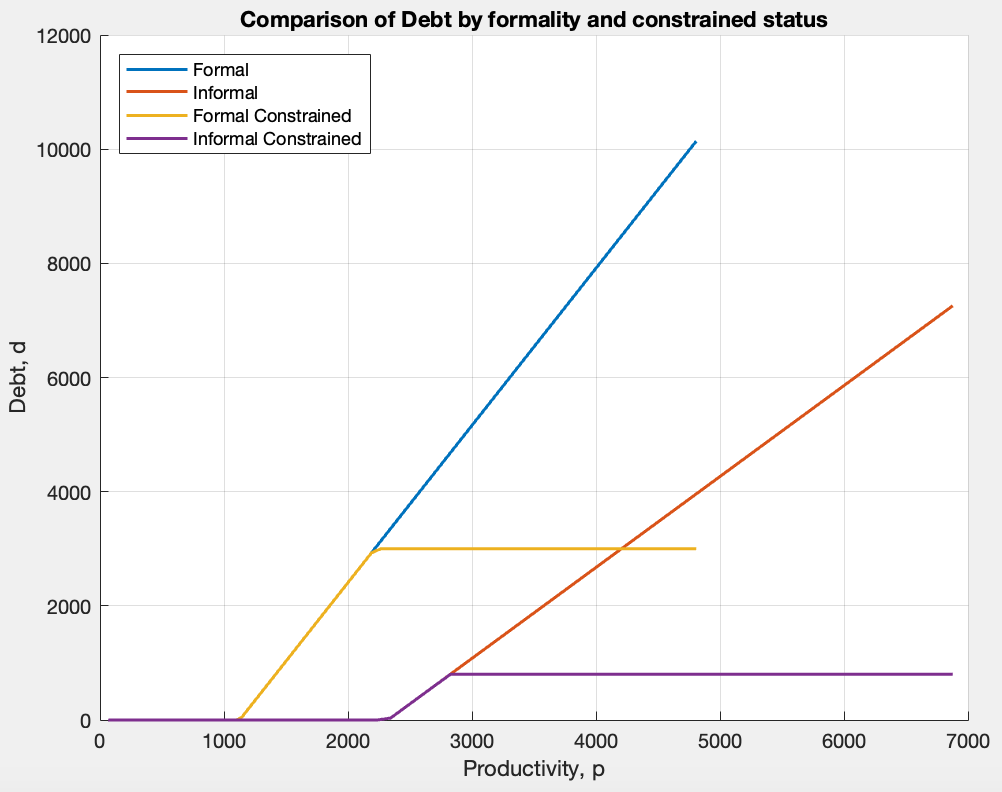
\includegraphics[scale=0.43]{debt_sim.png}
        \end{center}
    \end{column}

    \pause

    \begin{column}{0.5\textwidth} 
        \begin{center}
            \textbf{Capital}
        \end{center}
        \vspace{-5mm}
        \begin{center}
            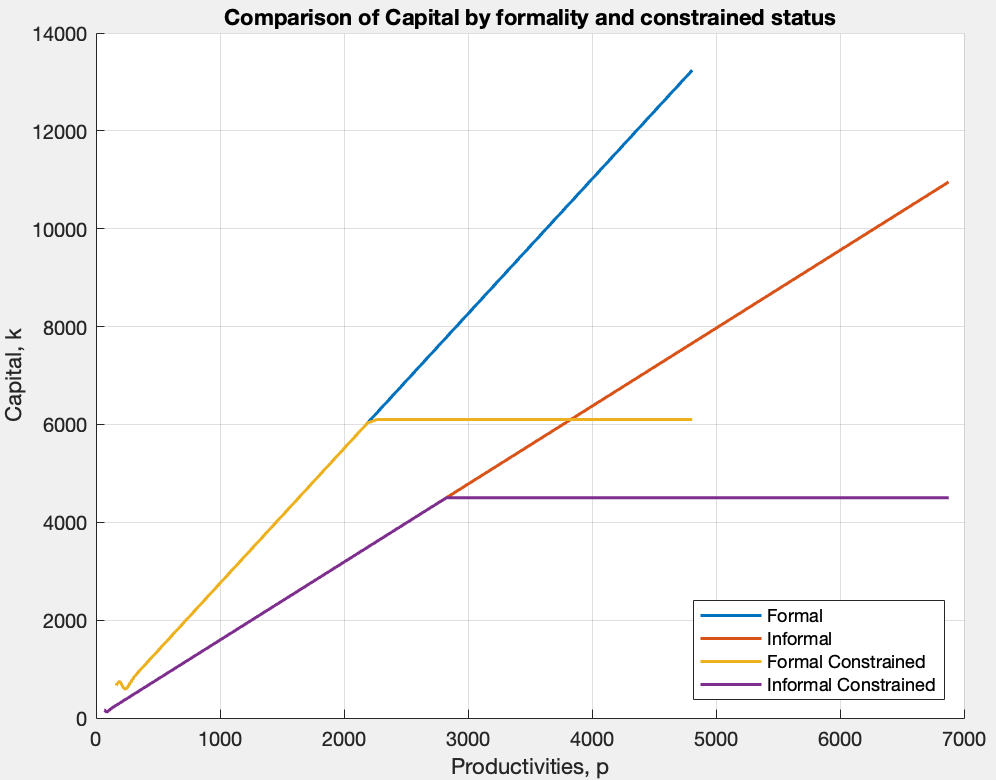
\includegraphics[scale=0.43]{capital_sim.png}
        \end{center}
    \end{column}
\end{columns}

\end{frame}

%------------------------------------------------

\begin{frame}
\frametitle{\textbf{Simulated model} 2/2}

\vspace{-10mm}

\begin{columns}[T] 
    \begin{column}{0.5\textwidth} 
        \begin{center}
            \textbf{Wages}
        \end{center}
        \vspace{-6mm}
        \begin{center}
            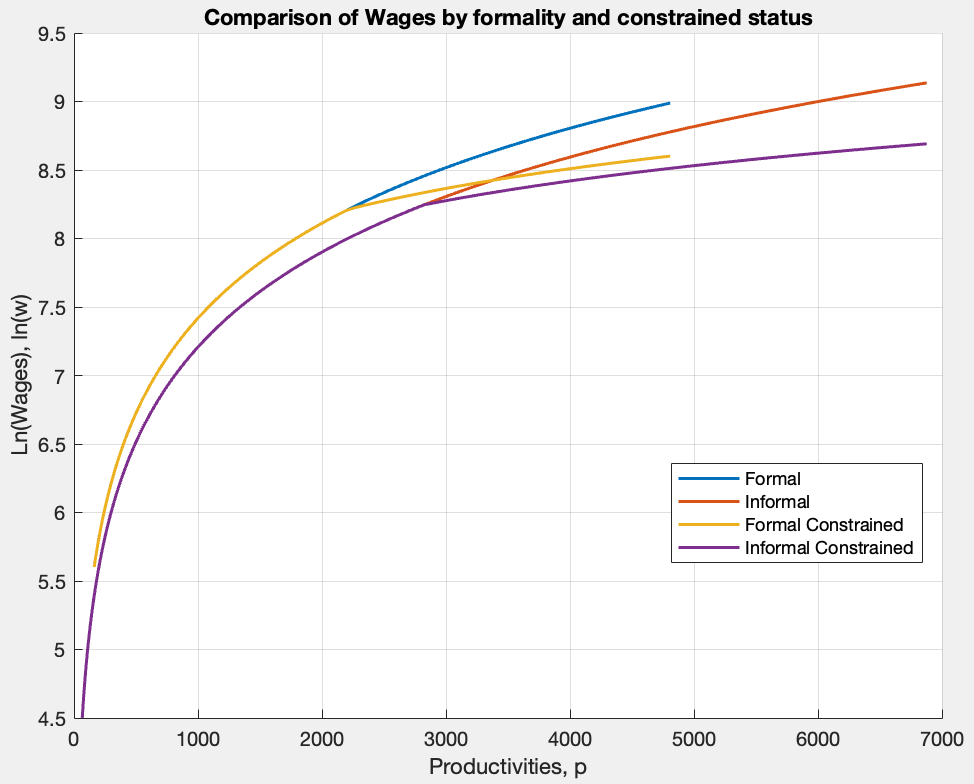
\includegraphics[scale=0.43]{wages_sim.png}
        \end{center}
    \end{column}

    \pause

    \begin{column}{0.5\textwidth} 
        \begin{center}
            \textbf{Profits}
        \end{center}
        \vspace{-6mm}
        \begin{center}
            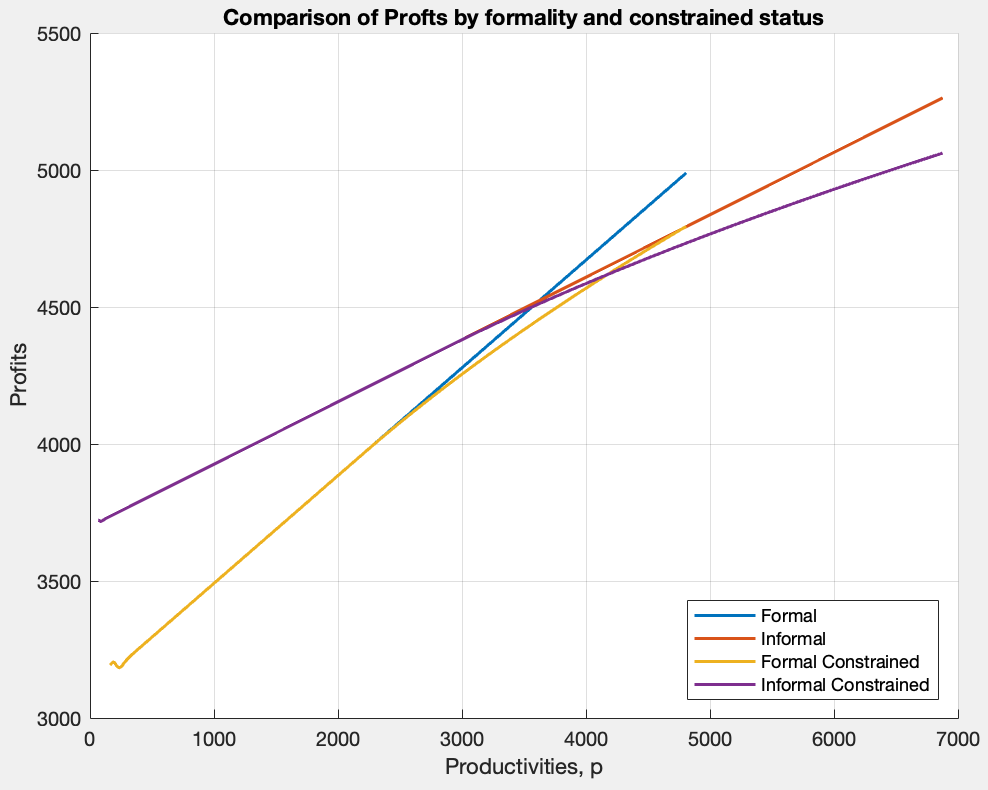
\includegraphics[scale=0.43]{profits_sim.png}
        \end{center}
    \end{column}
\end{columns}

\end{frame}

%------------------------------------------------

\begin{frame}
\frametitle{\textbf{Conclusion}}

\textbf{Model}: A search model extended with capital and informality decisions
\begin{itemize}
    \item \textbf{Simulation} w/preliminary parameters are consistent with the observational data.
    \begin{itemize}
        \item Informal firms use less capital, pay lower wages, are less productive and hold less credits.
        \item Capable of mapping financial frictions into capital, wages, and informality decisions.
    \end{itemize} 
\end{itemize}

\pause
\vspace{5mm}

\textbf{Empirical strategy}: Assessing causation of the observational evidence
\begin{itemize}
    \item Disentangle credit shocks to evaluate its effects on firms and LLM characteristics.
    \item A credit supply shock increases sales and workers but reduces small firms informality. 
\end{itemize}

\pause
\vspace{5mm}

\textbf{To do}: Motivational evidence and model
\begin{itemize}
    \item Estimate the model via GMM, and build the Hopenhayn model.
    \item Refine the motivational evidence with heterogeneous effects.
\end{itemize}

\pause
\vspace{5mm}

\textbf{Takeaway}: Informality is multi-factorial but credit friction is an important unexplored factor.
\begin{itemize}
    \item Policies affecting financial conditions can reduce informality \textit{extensively and intensively}.
\end{itemize}

\end{frame}

%------------------------------------------------

\begin{frame}[noframenumbering]
\frametitle{}
\begin{center}
    \LARGE T H A N K \quad Y O U ! \\
    \vspace{10mm}
    \LARGE david.morales@tse-fr.eu
\end{center}

\end{frame}

%------------------------------------------------

\begin{frame}[noframenumbering]
\frametitle{Standard deviation of shocks in selected years} \label{sdsy}

\begin{center}
    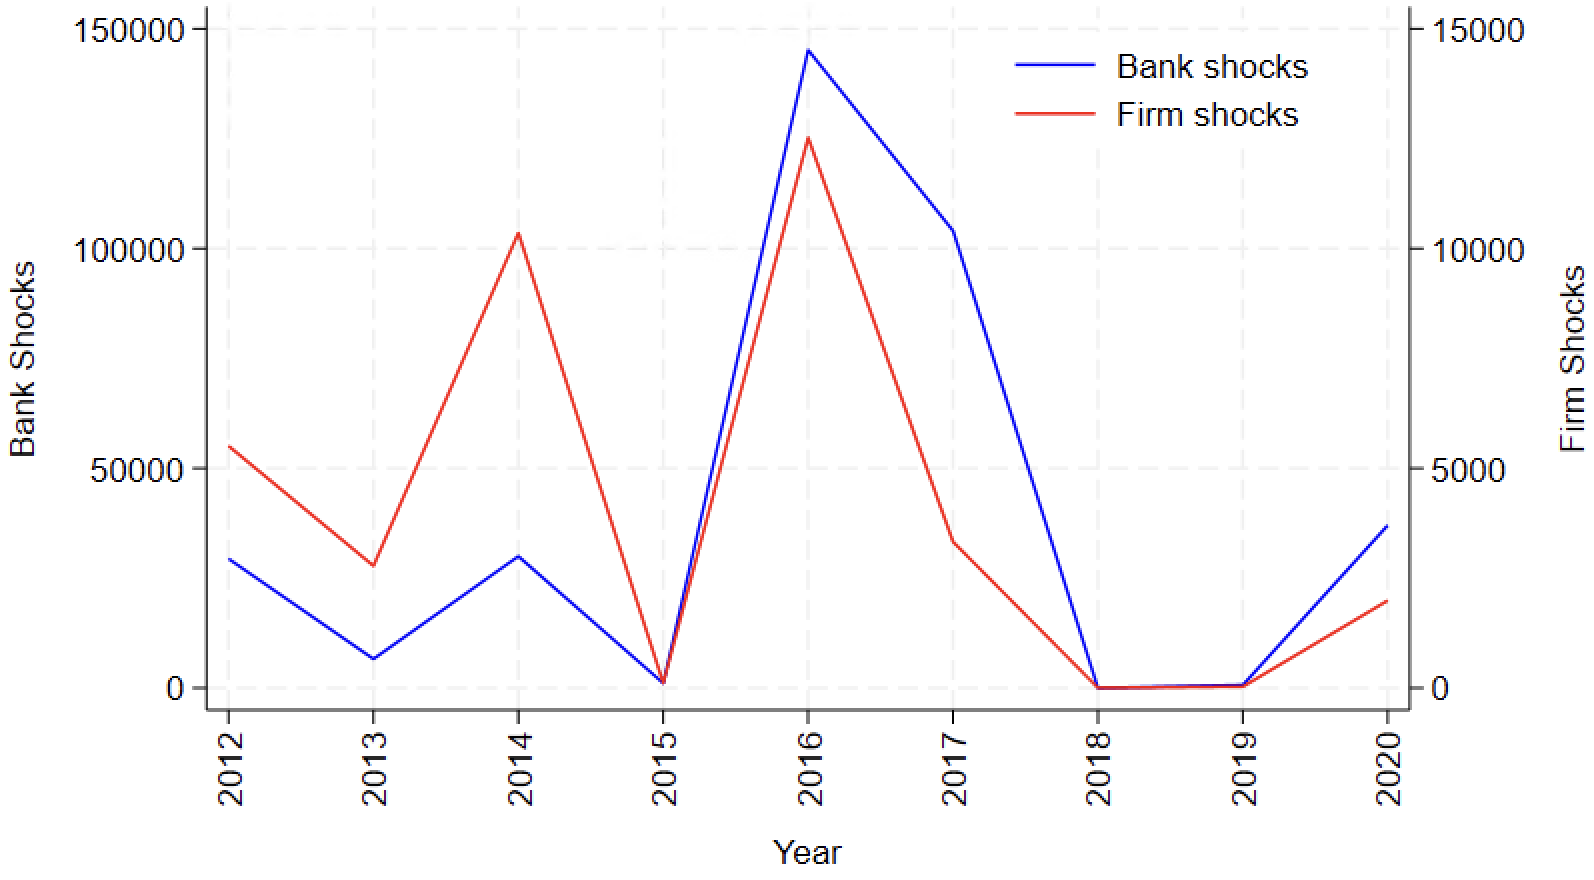
\includegraphics[scale=0.4]{SDshocksSY.png}
\end{center}

\hyperlink{back4}{\beamergotobutton{Back}}

\end{frame}

%------------------------------------------------

\begin{frame}[noframenumbering]
\frametitle{\textbf{References}} 

\tiny

\bibliographystyle{abbrvnat}
\bibliography{ref}

\end{frame}

%------------------------------------------------

\end{document}